\documentclass[11pt,a4paper]{article}
\author{TalentSprint}
\date{}
\usepackage{verbatim}
\usepackage{fancyhdr}           % For header and footer
\usepackage{multicol}
\usepackage{colortbl}           % For coloured tables
\usepackage{setspace}           % For line height
\usepackage{seqsplit}           % Splits long words.
\usepackage{amsmath} 
\usepackage{graphicx}
\usepackage{array}
\usepackage{enumitem}
\usepackage{xcolor}
\usepackage[tikz]{bclogo}
\usepackage{textcomp}
\usepackage{listings}
\lstset{language=python,numbers=left,numberstyle=\tiny,numbersep=10pt,showstringspaces=false}

\headheight=14pt
\lhead{\nouppercase{}}
\rhead{\nouppercase{\leftmark}}

\newcommand*\lstinputpath[1]{\lstset{inputpath=#1}}
\lstinputpath{../Code/}
\graphicspath{{../Images/} {../ScreenShots/}}

\setcounter{tocdepth}{1}
\setlength\parindent{0pt}
\parskip=4pt
\newcommand{\Code}[1]{\textbf{\texttt{#1}}}

% Lengths and widths
\addtolength{\textwidth}{5cm}
\addtolength{\hoffset}{-1cm}
\setlength{\headsep}{-12pt} % Reduce space between header and content
\setlength{\headheight}{85pt} % If less, LaTeX automatically increases it
\renewcommand{\footrulewidth}{2pt} % Remove footer line
\renewcommand{\headrulewidth}{1pt} % Remove header line
\renewcommand{\seqinsert}{\ifmmode\allowbreak\else\-\fi} % Hyphens in seqsplit
% This two commands together give roughly
% the right line height in the tables
\renewcommand{\arraystretch}{1.3}
\onehalfspacing

% Commands
\newcommand{\SetRowColor}[1]{\noalign{\gdef\RowColorName{#1}}\rowcolor{\RowColorName}} % Shortcut for row colour
\newcommand{\mymulticolumn}[3]{\multicolumn{#1}{>{\columncolor{white}}#2}{#3}} % For coloured multi-cols
\newcolumntype{x}[1]{>{\raggedright}p{#1}} % New column types for ragged-right paragraph columns
\newcommand{\tn}{\tabularnewline} % Required as custom column type in use

% Font and Colours
\definecolor{HeadBackground}{HTML}{333333}
\definecolor{FootBackground}{HTML}{666666}
\definecolor{TextColor}{HTML}{333333}
\definecolor{DarkBackground}{HTML}{6B8E23} %{FD1AA8}
\definecolor{LightBackground}{HTML}{E8FED8} %D3FDC8
\definecolor{tit}{HTML}{FF6600}
\renewcommand{\familydefault}{\sfdefault}
\color{TextColor}
 \headsep = 25pt
% Header and Footer
\pagestyle{fancy}
\usepackage[headheight=110pt]{geometry}
\fancyhf{}% Clear header/footer

\fancyhead[r]{
\includegraphics[width = 4cm, height = 2cm]{TS-Logo.png}\hspace{0cm}}

%=================================TITLE=====================================
\fancyhead[l]{\Large{\bf{\textcolor{tit}{\textrm{Recursion}}}}}
%===========================================================================

\renewcommand{\headrulewidth}{0.4pt}% Default \headrulewidth is 0.4pt
\renewcommand{\footrulewidth}{0.4pt}% Default \footrulewidth is 0pt

\rfoot{Page \thepage}
\lfoot{COPYRIGHT \textcopyright TALENTSPRINT, 2015. ALL RIGHTS RESERVED.}

\begin{document}


%\chapter{Recursion}

\section*{Recursive Functions}
A function that calls itself is known as recursive function and the process of a function calling itself is known as ``recursion''.

Recursion can be quite elegant;  requiring fewer variables which make the program clean. Recursion can be used to replace complex nesting code by dividing the problem into same problem of its sub-type. On other hand, it is hard to think the logic of a recursive function. It may be also difficult to debug the code containing recursion.

\subsection*{Example}
A function to factorial of `n' is follows
\begin{lstlisting}
  int fact(int n) {
    if (n <= 1) {
      return 1;
    } else {
      return n * fact (n - 1);
    }
  }
\end{lstlisting}

Assume n is 3; since it is not 1, the statement \texttt{fact = n * fact(n - 1);}  will  be executed with n = 3. The sequence of operations can be summarized as follows:
\begin{lstlisting}[numbers=none]
     return  3 * fact(2)
     return  3 * 2 * fact(1)
     return  3 * 2 * 1
\end{lstlisting}

\begin{quote}
  Every recursive function must have a terminating condition otherwise it may lead to infinite calls. In the above code, the termination condition occurs when n = 1 or n = 0 (1! = 1 and 0! = 1).
  \end{quote}

\subsection*{Attributes of recursive function}
\begin{enumerate}
\item A recursive function is a function which calls itself.
\item The recursive program may be slower because of stack overheads. 
\item The recursive program may consume more memory.
\item A recursive function must have recursive conditions, terminating conditions, and recursive expressions.
\end{enumerate}

\subsubsection*{Example}
This program prints the required term in the Fibonacci series using recursion. In the Fibonacci series, each term is the sum of the two preceding terms. The first few terms are: 0, 1, 1, 2, 3, 5, 8, \ldots

\lstinputlisting{Program-09-1.c}

\begin{figure}[ht]
\begin{center}
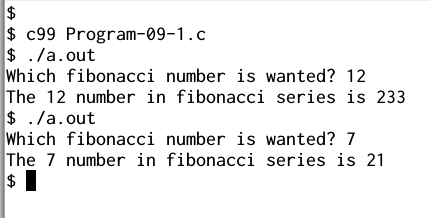
\includegraphics[scale=0.6]{Output-09-1.png}
\caption{Fibonacci Sequence}
\label{output-09-1}
\end{center}
\end{figure}

\begin{bclogo}[couleur=blue!5, arrondi=0.3, logo=\bctrombone]{Summary}
\begin{itemize}
\item Use recursion for \textbf{clarity}, and (sometimes) for a reduction in the time needed to write and debug code, not for space savings or speed of execution.
\item Remember that every recursive method must have  a \textbf{base case}
\item Also remember that every recursive method must make progress towards its base case.
\item Sometimes a recursive method has more to do following  a recursive call. It gets done only after the recursive call (and all calls it makes) finishes.
\item Recursion is often simple and elegant, can be efficient, and tends to be underutilized. Consider using recursion more!
\end{itemize}
\end{bclogo}
\end{document}